\section{(10) Приближенные алгоритмы для метрической задачи коммивояжера}

\begin{problem*}\textbf{(Метрическая задача коммивояжера, metric TSP).} Дан \textbf{полный} неориентированный граф с неотрицательными весами $l$ у ребер, удовлетворяющий неравенству треугольника: для любой тройки вершин $u, v, w$ верно $l(uv) + l(vw) \geq l(uw)$. Найти в нем цикл минимальной длины, проходящий по всем вершинам (минимальный гамильтонов цикл). \end{problem*}

\subsection{2-оптимальное решение}
\textbf{Решение (2-оптимальное).} Найдем $T$ -- минимальное остовное дерево в $G$. Удвоим в $T$ каждое ребро, получится эйлеров граф $D$. Пусть $C$ -- порядок вершин в эйлеровом цикле в $D$. Построим по нему гамильтонов цикл $A$ следующим образом: для всякой вершины $v$ удалим все ее вхождения в список $C$, кроме первого. Описание алгоритма закончено.

Два примера работы алгоритма на полных графах, заданных набором точек на плоскости:

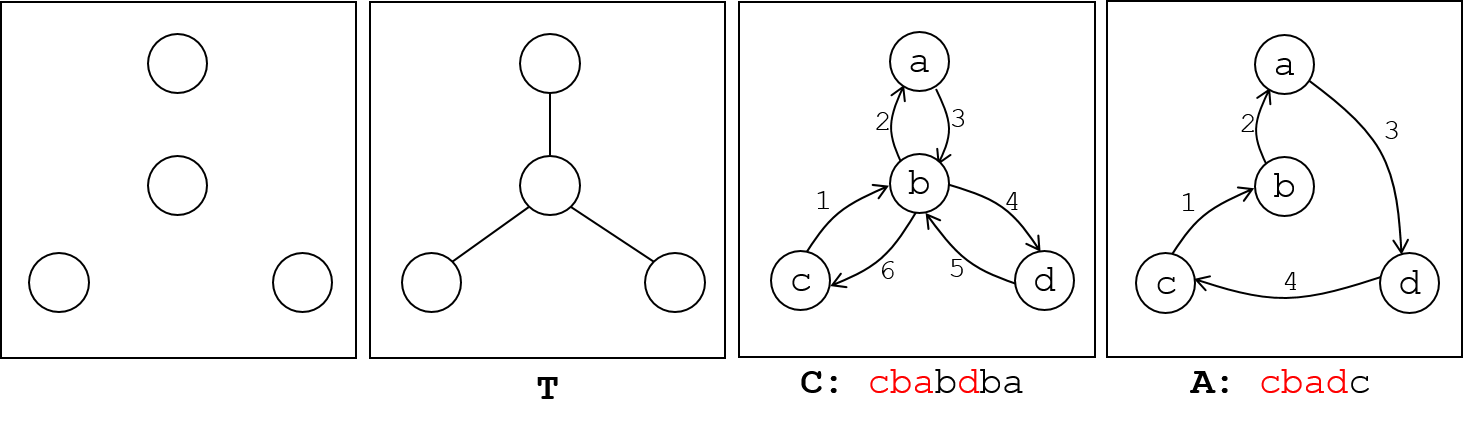
\includegraphics[width=\textwidth]{figures/ex_shorthamil.png} \\
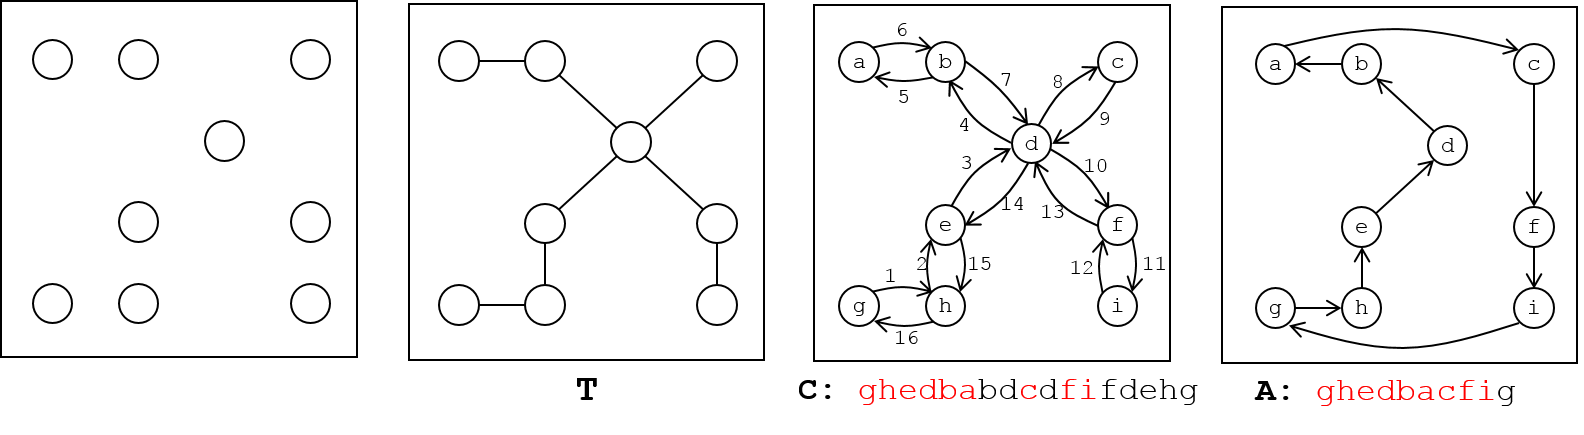
\includegraphics[width=\textwidth]{figures/ex_longhamil.png}

Обозначим $TSP$ -- вес оптимального гамильтонова цикла, $MST$ -- вес найденного минимального остовного дерева $T$.
\begin{theorem*} Вес $A$ $\leq 2 \cdot TSP$ \end{theorem*}
\begin{proof}
Заметим, что $MST \leq TSP$. Действительно, удалением любого ребра из гамильтонова цикла мы получаем какое-то остовное дерево, вес которого не превосходит $TSP$.

Вес эйлерова цикла $C$ по определению равен $2\cdot MST \leq 2\cdot TSP$. Вес $A$ не превосходит $C$, потому что при каждом удалении вершины суммарное расстояние неувеличивается по неравенству треугольника. Стало быть, вес $A \leq 2 \cdot TSP$.
\end{proof}

\subsection{1.5-оптимальное решение}

\textbf{Решение (1.5-оптимальное).} Найдем $T$ -- минимальное остовное дерево в $G$. Выделим все вершины нечетной степени в $T$, их четное число. Обозначим индуцированный (из $G$) граф на этих вершинах $O$. Этот граф все еще полный, значит в нем есть совершенное паросочетание. Пусть $M$ -- ребра минимального совершенного паросочетания в $O$. Добавим их в $T$ (если какое-то ребро $M$ уже есть в $T$, то добавим еще раз) -- получим граф $T'$, у которого степени всех вершин четные. Дальнейшие действия те же: пусть $C$ -- порядок вершин в эйлеровом цикле в $T'$, гамильтонов цикл $A$ строится по $C$ выкидыванием всех повторных вхождений всякой вершины. Описание алгоритма закончено.

Снова два примера работы алгоритма:

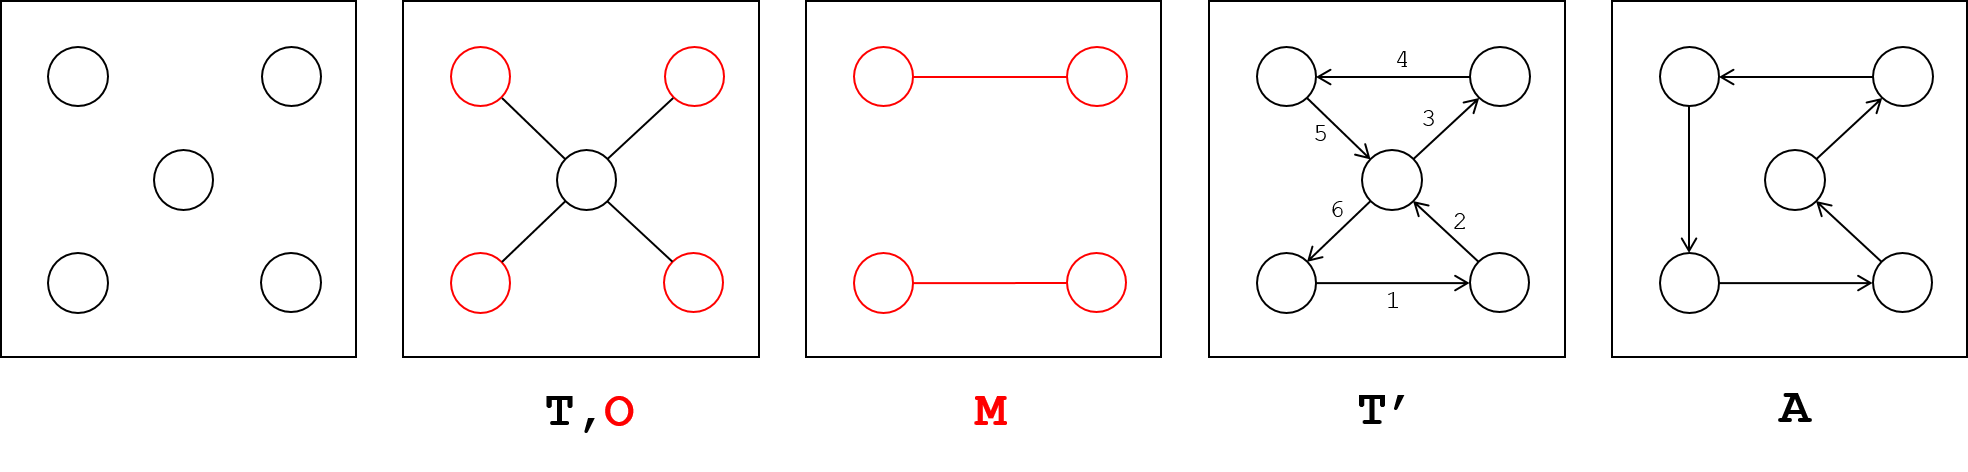
\includegraphics[width=\textwidth]{figures/ex_shorthamil2.png} \\
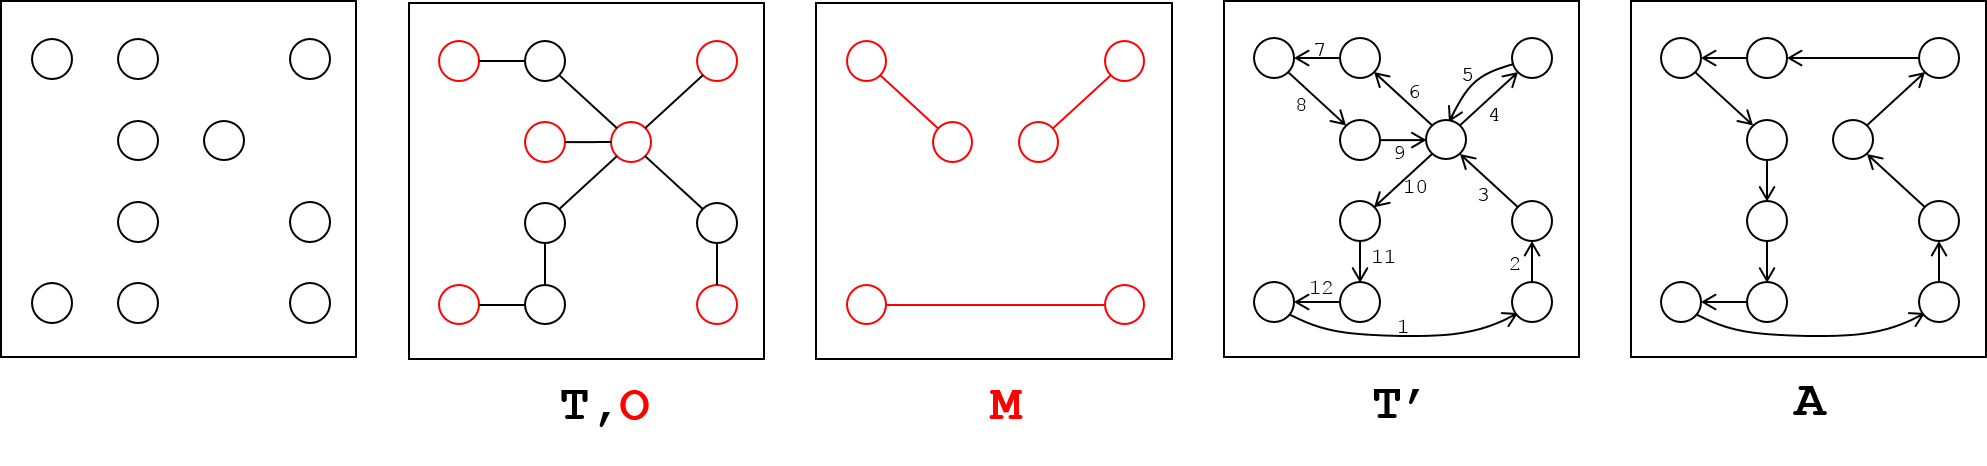
\includegraphics[width=\textwidth]{figures/ex_longhamil2.png}

Снова обозначим $TSP$ -- вес оптимального гамильтонова цикла, $MST$ -- вес остовного дерева $T$.

\begin{theorem*} Вес $A \leq \frac{3}{2}\cdot TSP$\end{theorem*}
\begin{proof}
По тем же рассуждениям (неравенство треугольника) вес найденного гамильтонова цикла $A$ не превосходит вес эйлерова графа $T'$, который равен $MST$ $+$ вес $M$, и по тем же рассуждениям $MST \leq TSP$. Достаточно показать, что вес $M \leq TSP/2$, а для этого в свою очередь достаточно доказать, что существует какое-то совершенное паросочетание на вершинах $O$ веса $\leq TSP/2$.

Мы построим это паросочетание так. Упорядочим вершины $M$ в том порядке, в котором они идут в \textbf{оптимальном} гамильтоновом обходе в $G$. Пусть $H$ -- гамильтонов цикл на вершинах $M$ в указанном порядке. Так как $H$ получен из оптимального гамильтонова цикла удалением вершин из него, то вес $H \leq TSP$. Далее, удалением из $H$ ребер через одно мы можем получить два различных совершенных паросочетания на вершинах $M$, причем их объединение есть в точности $H$. Сумма весов этих двух паросочетаний есть вес $H$, таким образом, хотя бы у одного из двух паросочетаний вес не превосходит $TSP/2$, что и требовалось.
\end{proof}
